\chapter{Risiko- und Anforderungsanalyse}
Dieser Bereich umfasst die durchgeführte Risikoanalyse für dieses Projekt. Die Risikoanalyse beinhaltet die Risikoidentifikation, die Risikokategorisierung und die Risikobehandlung. Im Anschluss an die Risikoanalyse wird die Anforderungsanalyse beschrieben, in der die funktionalen und nichtfunktionalen Anforderungen definiert werden. 
\section{Risikoanalyse} \label{RisikoAnalyse}
Um während der Entwicklung und Umsetzung des Projekts nicht von projektgefähr"-denden Risiken überrascht zu werden, wurde vor der Entwicklung eine Risikoanalyse durchgeführt und entsprechende Maßnahmen geplant. Die durchgeführte Risikoanalyse umfasst drei Bereiche; die Risikoidentifizierung, die Risikokategorisierung und die Risikobehandlung. Die Risikoidentifikation dient der Erfassung auftretender Risiken. Diese werden in der Risikokategorisierung analysiert und Risikoklassen zugeordnet, um die Auswirkung auf die Umsetzung festzustellen. In der Risikobehandlung werden anschließend für jedes Risiko entsprechende (Gegen-) Maßnahmen oder alternative Lösungsansätze geplant, die während der Umsetzung angewendet werden.\\
Für die Risikoanalyse wurden die einzelnen Komponenten des Projekts separat analysiert und die auftretenden Risiken identifiziert. Die benötigte/ verwendete Hardware dieses Projekts besteht aus den folgenden Komponenten:
\begin{itemize}
\item Das Ultraschallgerät/ Sonoscape, auf dem die Ultraschallbilder generiert werden.
\item Das mobile Endgerät, für das eine Anwendung zur Verarbeitung und Anzeige der Ultraschallbilder implementiert wird.
\item Die Halterung für die Befestigung des mobilen Endgerätes und des Teilerspiegels an der Ultraschallsonde.
\end{itemize}

\subsection{Risikoidentifizierung}
Die nachfolgende Tabelle \ref{tab:Risikoidentifizierung} umfasst die Voraussetzung/ Umsetzung, bei der entsprechende Risiken auftreten können. Insgesamt wurden elf Risiken ermittelt, die eine Realisierung des Projekts gefährden. Diese werden in der nachfolgenden Tabelle vorgestellt. Die Tabelle umfasst eine zugeordnete Risikoidentifikation (RisikoID), eine Beschreibung der Voraussetzung/ Umsetzung sowie das zugehörige Risiko. 

\begin{center}
\begin{table} [H]
\small
    \begin{tabular}{ | p{0.1\textwidth} | p{0.4\textwidth} | p{0.4\textwidth} |}
    \hline
   \textbf{RisikoID} &  \textbf{Voraussetzung/ Umsetzung} & \textbf{Risiko}\\
      \hline
      	1	
      & Zugriff auf das Betriebssystem wird für die Extraktion der Bilddaten und die Installation von zusätzlicher Software und Treibern benötigt. 	
      & Kann Zugriff auf das Betriebssystem erlangt werden? \\
      \hline
	  2	
	& Berechtigungen werden für die Installation von Software und Treibern auf dem Ultraschall benötigt.	
	& Sind ausreichend Berechtigungen auf dem Ultraschallgerät vorhanden? \\
	\hline
	3
	& Die benötigten Ultraschallbilder müssen extrahiert/ aufgenommen werden können.	
	& Kann auf die Bilddaten des Ultraschallgerätes zugegriffen werden? \\
	\hline
	4	
	& Die Netzwerkschnittstelle wird für die Übertragung der Bilddaten benötigt.	
	& Verfügt das Ultraschallgerät über eine Netzwerkschnittstelle? \\
	\hline
	5	
	& Die Netzwerkschnittstelle wird für die Übertragung der Bilddaten benötigt.	
	& Kann das Ultraschallgerät um eine Netzwerkkomponente erweitert werden? \\
	\hline
	6	
	& Die Übertragung der Ultraschallbilder im Ursprungsformat kann sich auf die Framerate (Anzahl der zu übertragenden Bilder) und die Performance auswirken.	
	& Können die Ultraschallbilder im Ursprungsformat in einem gewissen Zeitintervall übertragen werden? \\
	\hline
	7	
	& Es wird ausreichend Rechenleistung für die Komprimierung und Dekodierung der Bilddaten benötigt, um eine geringe Latenz bzw. die Echtzeitfähigkeit zu gewährleisten.	
	& Ist ausreichend Rechenleistung für die Realisierung in Echtzeit vorhanden? \\
	\hline
	8	
	& Es wird ausreichend Rechenleistung für die Dekodierung und die Bildverarbeitung benötigt.	
	& Ist ausreichend Rechenleistung für die Dekodierung der Bilddaten und die Bildverarbeitung vorhanden?\\
	\hline
	9	
	& Das mobile Endgerät muss für die Darstellung der Ultraschallbilder über eine ausreichende Auflösung, Helligkeit und eine geeignete Displaygröße verfügen.	
	& Ist eine realitätsgetreue Darstellung der Ultraschallbilder auf dem mobilen Endgerät möglich? \\
	\hline
	10	
	& Aufgrund der exakten Vorgabe der Ausrichtung der einzelnen Komponenten (Abstand, Winkel) muss eine Vorrichtung gebaut werden, auf der sich das mobile Endgerät und der Teilerspiegel befestigen lassen.	
	& Kann eine leichtgewichtige, starre und stabile Vorrichtung entworfen und umgesetzt werden? \\
	\hline
	11	
	& Die Vorrichtung muss  an einer festgelegten Stelle fixiert und befestigt werden, um eine exakte Überlagerung der Bilddaten mit der Realität zu realisieren.	
	& Kann die Vorrichtung an der Ultraschallsonde angebracht werden? \\
\hline
  
    \end{tabular}
     \caption{{\small Tabelle Risikoidentifizierung}}
     \label{tab:Risikoidentifizierung}
    \end{table}
\end{center}

\subsection{Risikokategorisierung}
In der Risikokategorisierung werden die identifizierten Risiken in bestimmte Risikoklassen eingeteilt und die Auswirkung auf die Umsetzung des Projekts festgestellt. Dies geschieht anhand der anzunehmenden Eintrittswahrscheinlichkeit und der dadurch entstehende Schaden durch die jeweiligen Risiken. Die Risikokategorisierung in der nachfolgenden Abbildung \ref{fig:risikokategorisierung} basiert auf der vorgestellten Methode von Marx \footcite{Risikomanagement}. Der Schaden bezieht sich in diesem Projekt auf die Einhaltung von Meilensteinen, die Realisierung des Projekts sowie die Qualität und Performance der gesamten Umsetzung. Die Kategorien unterteilen sich dabei in drei unterschiedliche Klassen, die in der nachfolgenden Abbildung wie folgt dargestellt werden:
\begin{itemize}
\item ROT  = projektgefährdend
\item GELB = kritisch
\item GRÜN = unkritisch
\end{itemize}
Von den ermittelten elf Risiken haben sieben Risiken eine projektgefährdende Auswirkung. Diese Risiken wurden daher mit einer hohen Priorität versehen und früh"-zeitig während der Projektrealisierung behandelt. Für alle Risiken wurden entsprechende Maßnahmen bzw. alternative Lösungen entworfen, die eine Projektumsetzung ermöglichen oder die Auswirkungen eines Risikos minimieren (siehe Kapitel \ref{Risikobeh}). 
\begin{figure}[H]
	\centering
	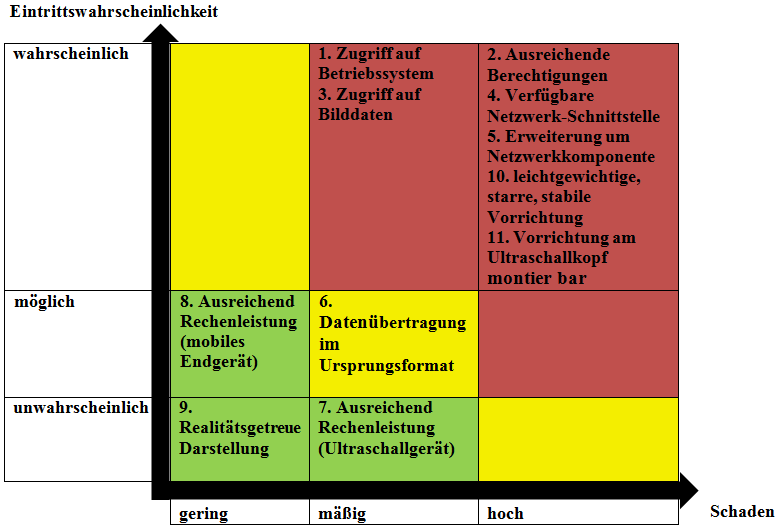
\includegraphics[width=1\textwidth]{Bilder/Risiko_und_Anforderungsanalyse/Risikokategorisierung.png}
	\caption{Risikokategorisierung}
	\label{fig:risikokategorisierung}
\end{figure}

\subsection{Risikobehandlung} \label{Risikobeh}
Für jedes identifizierte Risiko wurden entsprechende Maßnahmen geplant, die im Laufe der Projektrealisierung umgesetzt wurden. Hierbei ging es vor allem um die Beschaffung des Zugriffs auf das Ultraschallgerät, die Installation von benötigten Treibern und zusätzlicher Software, die Extraktion der Ultraschallbilder, der Netzwerkzugriff des Ultraschallgeräts und die Konstruktion einer stabilen Halterung, die an der Ultraschallsonde befestigt werden kann. Die entsprechenden Maßnahmen reichten hierbei von der Konsultation und Kommunikation mit dem Gerätehersteller über die Analyse der beteiligten Komponenten bis hin zur Umsetzung von Prototypen während der Planung und der Realisierung des Projektes. \\ 
Zu beginn des Projekts wurde ein Projektplan erstellt, der aus Übersichtlichkeits"-gründen nicht komplett angezeigt wird, dieser ist aber im Anhang zu finden (siehe \ref{AnhangA}). Der entwickelte Projektplan umfasst fünf Hauptbereiche, in denen die verschiedenen Arbeitsschritte für das Projektteam festgelegt  und während der Projektdurchführung umgesetzt wurden. Die fünf Hauptbereiche bestehen aus: 
\begin{enumerate}
\item der Recherche und der Vorbereitung,
\item dem Eignungstest des vorhandenen Ultraschallgerätes,
\item dem Entwurf und der Umsetzung der Halterung,
\item die Implementierung 
	\begin{enumerate}
         \item der Serversoftware,
         \item der Clientsoftware
	\end{enumerate}
\item und der Evaluierung
\end{enumerate}

Diese Hauptbereiche umfassen insgesamt 44 weitere Arbeitspakete, in denen die Umsetzung strukturiert und geplant wurde. In der nachfolgenden Tabelle \ref{tab:Risikomassnahmen} sind die zugehörigen Arbeitspakete sowie die geplanten Maßnahmen angegeben, die durchgeführt wurden.

\begin{center}
\begin{minipage}{1\textwidth}
\begin{table} [H]
\small
    \begin{tabular}{ | p{0.1\textwidth} | p{0.5\textwidth} | p{0.3\textwidth} | } 
    \hline
   \textbf{RisikoID} &  \textbf{Maßnahme(n)} & \textbf{Arbeitspaket(e)} \\
      \hline
1	&Konsultation und Kommunikation mit dem Gerätehersteller	& Systemzugriff (4) \\
\hline
2	&Analyse vorhandener bzw. Erweiterung der Berechtigungen des Ultraschallgeräts	& Berechtigungen prüfen (5)	\\
\hline
3	&Analyse der Zugriffsmöglichkeiten auf den internen Bildspeicher oder Installation und Ausführung zusätzlicher Software	& Zugriffsmöglichkeiten Bildspeicher prüfen (6)	\\
\hline
4	&Vorhandene Schnittstellen des Ultraschallgeräts analysieren. 	& Netzwerkzugriff prüfen (7)	\\
\hline
5	&Die Möglichkeiten für die  Installation einer zusätzlichen Netzwerkschnittstelle überprüfen (zusätzliche Hardware: Router, WLAN- Stick)	& Netzwerkzugriff prüfen (7)	\\
\hline
6	&Um den zu übertragenden  Datenumfang zu reduzieren, muss ggf. eine Komprimierung der Daten erfolgen.	& Serversoftware implementieren (16)
	\\
\hline
7	&Analyse der benötigten Rechenleistung 	& Serversoftware (21)/ Clientsoftware (28) implementieren	\\
\hline
8	&Analyse der benötigten Rechenleistung und Beschaffung eines mobilen Endgerätes mit genügend Rechenleistung	& geeignetes Smartphone auswählen (2)	\\
\hline
9	&Festlegen der benötigten Auflösung und der Displaygröße	& geeignetes Smartphone auswählen (2)	\\
\hline
10	&Planung der Vorrichtung,
Analyse der benötigten Materialen, Prototyping	& Halterung/ Hardware konstruieren (11)	\\
\hline
11	&Prototyping	& Halterung/ Hardware konstruieren (11)	\\
\hline
     \end{tabular}
     \caption{{\small Tabelle Risikomaßnahmen}}
     \label{tab:Risikomassnahmen}
     \end{table}
     \end{minipage}
\end{center}

\section{Anforderungsanalyse}  \label{AnfAnalyse}
Die Anforderungsanalyse umfasst die Definition der funktionalen und der nichtfunktionalen Anforderungen für das Projekt. Im folgenden Abschnitt 2.2.1 werden die funktionalen Anforderungen für die einzelnen Bereiche „Sonoscape/ Ultraschallgerät“, „Datenübertragung“, „mobile Applikation“, „Bildverarbeitung“ und die „grafische Benutzeroberfläche“ festgelegt. Die nichtfunktionalen Anforderungen in Abschnitt 2.2.2 umfassen die Bereiche "mobiles Endgerät", "Halterung\grqq und "Darstellung der Ultraschallbilder". In diesen Abschnitten werden die  Funktionalitäten definiert, welche die gesamte Anwendung erfüllen „muss“ (absolute Gültigkeit), „soll“ (Empfehlung) oder „kann“ (optional).   
\subsection{Funktionale Anforderungen} \label{FunkAnf}
\begin{minipage}{\textwidth}
Sonoscape/ Ultraschallgerät
\begin{itemize}
\item Das erstellte Ultraschallbild muss in derselben Auflösung extrahiert werden können, in der es vom Ultraschallgerät generiert wurde.
\item Das Ultraschallgerät muss um eine Netzwerkkomponente für den Netzwerkzugriff ergänzt werden.
\item Das Sonoscape muss um eine Serverfunktionalität ergänzt werden, über die die Ultraschallbilder übertragen werden.
\item Die extrahierten Bilder/ Frames des Ultraschallgerätes müssen vor der Übertragung in ein entsprechendes Format konvertiert werden.\\
\end{itemize}
\end{minipage}

\begin{minipage}{\textwidth}
Datenübertragung
\begin{itemize}
\item Um die zu übertragenden Daten zu verringern, muss eine Datenkomprimierung durchgeführt werden. 
\item Die Datenübertragung muss durch einen IO-Service realisiert werden.
\item Die Ultraschallbilder müssen kontinuierlich separat übertragen werden.
\item Die Ultraschallbilder müssen mit einer konstanten Framerate zw. 12-30 Frames per second (fps) übertragen und angezeigt werden. Die Variabilität der Framerate ist abhängig von der Anzahl der erzeugten Ultraschallbilder durch das Ultraschallgerät. 12 Frames werden von dem Gerät erzeugt, wenn zusätzliche Informationen in den Bildern angezeigt werden (bspw. Doppler Effekt), 30 Frames hingegen werden bei der normalen Verwendung ohne zusätzliche Informationen erzeugt.
\item Das Protokoll für die Datenübertragung muss TCP/IP sein.
\end{itemize}
\end{minipage}

\begin{minipage}{\textwidth}
Mobile Applikation
\begin{itemize}
\item Die mobile Applikation muss eine Verbindung zum Server aufbauen.
\item Die mobile Applikation muss über einen festgelegten Port auf eingehende Daten lauschen.
\item Die mobile Applikation muss die Konvertierung des ankommenden Bytestreams in ein entsprechendes Format durchführen.
\item Die verarbeiteten Frames müssen auf der Benutzeroberfläche angezeigt werden. Anschließend müssen die Frames gelöscht werden und der belegte Speicherplatz wieder freigegeben werden. 
\item Bei der Verwendung der mobilen Applikation kann der Benutzer über einen Verbindungsabbruch oder einen Datenverlust informiert werden.\\
\end{itemize}
\end{minipage}

\begin{minipage}{\textwidth}
Bildverarbeitung
\begin{itemize}
\item Die Bildverarbeitung muss innerhalb der mobilen Anwendung realisiert werden.
\item Die Bildverarbeitung muss die relevanten Informationen des Ultraschallbildes durch das Ausschneiden und die Zusammensetzung eines neuen Frames bereitstellen.\\
\end{itemize}
\end{minipage}

\begin{minipage}{\textwidth}
Die grafische Benutzeroberfläche
\begin{itemize}
\item Die Benutzeroberfläche der mobilen Applikation muss einheitlich und simpel aufgebaut sowie intuitiv benutzbar sein, um bei der Verwendung während einer Ultraschalluntersuchung nicht abzulenken.
\item Auf der grafischen Benutzeroberfläche müssen die Ultraschallbilder kontinuierlich angezeigt werden.
\end{itemize}
\end{minipage}
\subsection{Nichtfunktionale Anforderungen} \label{NichtFunkAnf}
\begin{minipage}{\textwidth}
Mobiles Endgerät
\begin{itemize}
\item Die Lichtdichte (Helligkeit) des Displays muss min. 500 cd/m² betragen.
\item Die Auflösung muss min. 1920x 1080 (Full HD) betragen.
\item Die Größe des Displays muss min. 5.0 Zoll betragen.
\item Das Gewicht soll höchstens 400 Gramm betragen.
\item Das Gerät muss über eine Netzwerkschnittstelle (WLAN (802.11)) verfügen.
\item Das Gerät muss über einen Beschleunigungssensor und ein Gyroskop verfügen.
\item Das Gerät muss über ausreichend Rechenleistung für die Bilddecodierung, Bildverarbeitung, Bildanzeige verfügen und min. vier Kerne (Quad-Core) besitzen.
\item Das Gerät muss auf einem offenen Betriebssystem basieren, für das unentgeltlich Programme implementiert und installiert werden können.\\
\end{itemize}
\end{minipage}

\begin{minipage}{\textwidth}
Halterung
\begin{itemize}
\item Es müssen nahezu identische Lichtverhältnisse auf beiden Seiten des Teilerspiegels existieren. Evtl. kann dazu eine zusätzliche Lichtquelle installiert werden.
\item Das Gewicht der kompletten Halterung (mobiles Endgerät, Teilerspiegel, Material zur Befestigung)  soll 500 Gramm nicht überschreiten.
\item Um den festgelegten Winkel zw. mobilem Endgerät, dem Teilerspiegel und der Sonde nicht zu verändern muss ein starres Material verwendet werden.\\
\end{itemize}
\end{minipage}

\begin{minipage}{\textwidth}
Darstellung der Ultraschallbilder
\begin{itemize}
\item Da nicht alle dargestellten Informationen des Ultraschallgerätes auf dem Ursprungsbild benötigt werden, müssen die benötigten Informationen aus dem Ursprungsbild ausgeschnitten und zu einem neuen Bild zusammengefügt werden.
\item Um die komplette Darstellung des Ultraschallbildes zu erfassen muss die Zoomstufe eins auf dem Ultraschallgerät ausgewählt sein.
\end{itemize}
\end{minipage}
